\vspace*{1em}

{\bf \large What is Complex Analysis?} The main object of study is a \cdef{holomorphic} function $f: G \to \cc$, where $G \subseteq \cc$. Namely, a function for which the limit
\[\lim_{h\to 0}\frac{f(z+h) - f(z)}{h}\]
exists and is finite on an open set; that is, a \cdef{complex\text{-}differentiable\  function} on an open set. As a set, $\cc = \rr^2$, so one can naively expect the theory to be similar to that of real analysis, in this case the behaviour of differentiable functions. Interestingly, the requirement of holomorphicity can yield results that have no counterpart in the real case.\\
\\
A prime example of this is \emph{Louiville's Theorem. Every bounded holomorphic function is constant.}

\vspace{1em}

\begin{discussion}
We begin with first addressing the existence and nature of $\cc$ itself. Let $\rr$ denote the (field of) real numbers. One immediately deduces that the equation
\begin{equation*}\label{imaginary}
x^2 + 1 = 0\tag{$*$}
\end{equation*}
has no solution in the real numbers. The (field of) complex numbers $\cc$ stems from our desire to find a set containing $\rr$ that extends the algebraic operations of addition and multiplication of real numbers and which contains not only solutions to the polynomial equation above but solutions to all polynomial equations.\\[0.5em]
Surprisingly enough, the construction amounts to defining a symbol $i$ that is a solution to (\ref{imaginary}) and then considering all expressions of the form
\[x + iy,\quad x,y \in \rr\]
\end{discussion}

\vspace*{2em}

\begin{mdframed}[backgroundcolor=paleyellow,linewidth=1pt]
\begin{center}
{\sc\Large Part I. Preliminaries}
\end{center}
\end{mdframed}

\begin{mdframed}
\begin{center}
{\Large Construction of the (field of) Complex Numbers}
\end{center}
\end{mdframed}

\begin{definition}[The set of Complex Numbers]
A \cdef{complex\ number} $z$ is simply an order pair $z \coloneqq (x,y)$ of real numbers. Thus, the set of all complex numbers is given by
\[\cc \coloneqq \rr^2 = \setp{(x,y)}{x,y\in \rr}\]
If $z = (x,y)$ is a complex number, then we call 
\[\Re z \coloneqq x \quad \text{and} \quad \Im z \coloneqq y\]
the \cdef{real} and \cdef{imaginary\ parts} of $z$ respectively.\\[0.5em]
Two complex numbers $z_1$ and $z_2$ are equal if and only if $\Re z_1 = \Re z_2$ and $\Im z_1 = \Im z_2$.\\
\\
If $\Re z = 0$ and $\Im z \neq 0$, we say that $z$ is \cdef{purely\ imaginary}. The set of purely imaginary complex numbers corresponds to the $y$-axis and is called the \cdef{imaginary\ axis} in $\cc$.
\end{definition}

%\vspace*{1em}

\begin{definition}[Binary Operations on $\cc$]
Let $z_1 = (x_1,y_1)$ and $z_2 = (x_2,y_2)$ be complex numbers. Then their \emph{sum} is
\[z_1 + z_2 = (x_1,y_1) + (x_2,y_2) \coloneqq (x_1 + x_2,y_1 + y_2)\]
and their \emph{product} is 
\[z_1 \cdot z_2 = (x_1,y_1) \cdot (x_2,y_2) \coloneqq (x_1x_2 - y_1y_2, x_1y_2 + x_2y_1)\]
\end{definition}

\vspace*{1em}

\begin{proposition}
There exists a subset of $\cc$ that is algebraically indistinguishable from $\rr$.
\end{proposition}
\begin{proof}
Consider the set (the $x$-axis)
\[\rr \times \set{0} = \setp{(x,0)}{x\in \rr} \subseteq \cc.\]
There is a bijection
\[\phi:\rr \to \rr \times \set{0},\ x \mapsto (x,0).\]
Moreover, 
\begin{align*}
\phi(x) + \phi(y) &= (x,0) + (y,0) = (x+y,0) = \phi(x+y)\\[0.5em]
\phi(x)\cdot\phi(y) &= (x,0)\cdot (y,0) = (xy - 0\cdot 0,x\cdot 0 + y\cdot 0) = (xy,0) = \phi(xy)\\[-2.5em]
\end{align*}
\end{proof}
According to the proposition, the operations of addition and multiplication on complex numbers we have defined extend the operations of addition and multiplication of real numbers. We therefore call the $x$-axis, the \cdef{real\ axis}.

\vspace*{1em}

\begin{discussion}
We identify each complex number $(x,0)$ with the corresponding real number $x$; more than that, abusing notation, we write
\[1 = (1,0)\quad \text{and} \quad (x,0) = x(1,0) = x\]
Now, define the \cdef{imaginary\ unit} $i \coloneqq (0,1)$. Then
\[i^2 = i\cdot i = (0,1)\cdot (0,1) = (0^2 - 1^2,1\cdot 0 + 1\cdot 0) = (-1,0) = -1.\]
Moreover, for any $z = (x,y) \in \cc$ we see that
\begin{align*}
z &= (x,y)\\[0.5em]
&= (x,0) + y(0,1) = x + iy = \Re z + i\Im z
\end{align*}
Hence, with our new notation
\[\cc = \setp{x+iy}{x,y\in \rr,\ i^2 = -1}\]
and
\begin{align*}
z_1 + z_2 = (x_1 + iy_1) + (x_2 + iy_2) &= (x_1 + x_2) + i(y_1 + y_2)\\[0.5em]
z_1 \cdot z_2 = (x_1 + iy_1) \cdot (x_2 + iy_2) &= (x_1x_2 - y_1y_2) + i(x_1y_2 + x_2y_1)
\end{align*}\\
Although we have expanded the real numbers and we will see that the complex numbers have several new and familiar properties. We do end up losing one property of the real numbers when working with complex numbers: total ordering (that extends the one on $\rr$ or is compatible with multiplication). In the world of complex numbers, it no longer makes sense to ask if $z_1 > z_2$ (see Problem \ref{prob 1.6}).
\end{discussion}

%\vspace*{1em}

In practice, the product of complex numbers can be computed by multiplying the expressions as if they were polynomials in the variable $i$, and using $i^2 = -1$. The fact that this works is left as Problem \ref{prob 1.2}.
\begin{example}
Compute $(1+i)(1-3i)$.
\end{example}
\begin{proof}[Answer]
We note
\begin{align*}
(1 + i)(1 - 3i) &= (1 - 3i) + i(1 - 3i)\\[0.5em]
&= (1 - 3i) + (i - 3i^2)\\[0.5em]
&= (1 - 3i) + (i + 3) = 4 - 2i\\[-2.5em]
\end{align*}
\end{proof}

\vspace*{1em}

\begin{proposition}[Algebraic Properties of $(\cc,+,\ \cdot\ )$]\label{cafield}\hfill
\begin{itemize}
\item[(1)] \emph{Additive Identity.} For every $z \in \cc$
\[z + 0 = z = 0 + z\]
\item[(2)] \emph{Associativity of Addition.} For every triple $z_1,z_2,z_3 \in \cc$
\[z_1 + (z_2 + z_3) = (z_1 + z_2) + z_3\]
\item[(3)] \emph{Commutativity of Addition.} For every pair $z_1,z_2 \in \cc$
\[z_1 + z_2 = z_2 + z_1\]
\item[(4)] \emph{Additive Inverses.} For every $z \in \cc$, there exists a complex number, denoted $-z$, such that
\[z + (-z) = 0 = (-z) + z\]
In fact, $-z \coloneqq (-1)z$, which is described in Problem \ref{prob 1.1}.
\item[(5)] \emph{Multiplicative Identity.} For every $z \in \cc$
\[z \cdot 1 = z = 1 \cdot z\]
\item[(6)] \emph{Associativity of Multiplication.} For every triple $z_1,z_2,z_3 \in \cc$
\[z_1 \cdot (z_2 \cdot z_3) = (z_1 \cdot z_2) \cdot z_3\]
\item[(7)] \emph{Commutativity of Multiplication.} For every pair $z_1,z_2 \in \cc$
\[z_1\cdot z_2 = z_2\cdot z_1\]
\item[(8)] \emph{Multiplicative Inverses.} For every $z \in \cc^* \coloneqq \cc\setminus\set{0}$, there exists a complex number, denoted $z^{-1}$ or $1/z$, such that
\[z \cdot z^{-1} = 1 = z^{-1} \cdot z\]
In fact, if $z =  x + iy$, then $z^{-1} = \dfrac{1}{z} \coloneqq \dfrac{x}{x^2 + y^2} - i\ \dfrac{y}{x^2 + y^2}$.
\item[(9)] \emph{Distributive Law.} For every triple $z_1,z_2,z_3 \in \cc$
\[(z_1 + z_2)\cdot z_3 = z_1\cdot z_3 + z_2\cdot z_3\]
\end{itemize}
\end{proposition}
\begin{proof}
(1) - (7) and (9) are left as Problem \ref{prob 1.3}. One proves these directly by showing that the left hand side matches the right hand side.
\begin{itemize}
\item[(8)] We note that
\begin{align*}
z\cdot\frac{1}{z} &= (x + iy)\left(\frac{x}{x^2 + y^2} - i\ \frac{y}{x^2 + y^2}\right)\\[1em]
&= (x + iy)\left(\frac{x}{x^2 + y^2} + i\ \frac{(-y)}{x^2 + y^2}\right)\\[1em]
&= \left(x\cdot\frac{x}{x^2 + y^2} - y\cdot\frac{(-y)}{x^2 + y^2}\right) + i\left(x\cdot\frac{(-y)}{x^2 + y^2} + y\cdot\frac{x}{x^2 + y^2}\right)\\[1em]
&= \left(\frac{x^2}{x^2 + y^2} + \frac{y^2}{x^2 + y^2}\right) + i\left(\frac{-yx + xy}{x^2 + y^2}\right)\\[1em]
&= \frac{x^2 + y^2}{x^2 + y^2} + i\cdot 0\\[1em]
&= 1
\end{align*}
Of course, we should comment that $z = (x,y) \neq (0,0)$ if and only if $x^2 + y^2 \neq 0$ (one proves this by stating and proving the contrapositive).
\end{itemize}
\vspace*{-\baselineskip}
\end{proof}

\vspace*{1.5em}

\begin{remark}
In the language of algebra, 
\begin{itemize}[leftmargin=*]
\item (1) -- (4) tells us that $(\cc,+)$ is an abelian group.
\item (5) -- (8) tells us that $(\cc^*,\ \cdot\ )$ is an abelian group.
\item (1) -- (9) tells us that $(\cc,+,\ \cdot\ )$ is a field.
\end{itemize}
\end{remark}

\vspace*{1.5em}

\begin{definition}
Consider $z_1,z_2 \in \cc$. We define \emph{subtraction} and \emph{division} as follows, respectively:
\begin{align*}
z_1 - z_2 &\coloneqq z_1 + (-z_2)\\[0.5em]
\dfrac{z_1}{z_2} &\coloneqq z_1\cdot z_2^{-1} = z_1\cdot \left(\dfrac{1}{z_2}\right),\quad z_2 \neq 0
\end{align*}
Writing down $z_1/z_2$ as $x+ iy$ is not easy to remember, one obtains it by a method akin to "rationalising the denominator", in this case we could call it "realifiying the denominator"
\[\frac{z_1}{z_2} = \frac{x_1 + iy_1}{x_2 + iy_2}\cdot \frac{x_2 - iy_2}{x_2 - iy_2}\]
This method will be clarified soon when we talk about conjugates and absolute value.
\end{definition}

%\vspace*{2em}

\begin{mdframed}
\begin{center}
{\Large Geometric Properties of Complex Numbers}
\end{center}
\end{mdframed}

As a set, we have $\cc = \rr^2$, so it's natural to visualise complex numbers as points in the \cdef{complex\ plane} (also called the \cdef{Argand\ plane}).
\[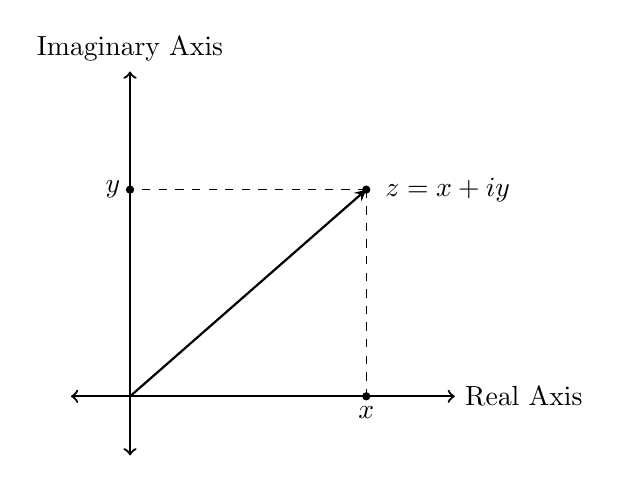
\begin{tikzpicture}[scale=0.75]
    \draw[<->,thick] (-1,0)--(5.5,0) node[right]{Real Axis};
	\draw[<->,thick] (0,-1)--(0,5.5) node[above]{Imaginary Axis};
	\draw[dashed] (4,3.5)--(0,3.5);
	\draw[dashed] (4,3.5)--(4,0);
    \fill (4,3.5) circle (2pt) node[right]{\ $z = x+iy$};
    \fill (0,3.5) circle (2pt) node[left]{$y$};
    \fill (4,0) circle (2pt) node[below]{$x$};
    \draw[->,>=stealth,thick] (0,0) -- (4,3.5);
  \end{tikzpicture}\]
Geometrically, addition of complex numbers is just the addition of the corresponding vectors in the euclidean plane. We will soon see a geometric interpretation of multiplication.

\[\begin{tikzpicture}[scale=0.75]
    \draw[<->,thick] (-1,0)--(5.5,0) node[right]{Real Axis};
	\draw[<->,thick] (0,-1)--(0,5.5) node[above]{Imaginary Axis};
    \fill[newblue] (6,4.5) circle (2pt) node[right]{\ $z_1 + z_2$};
    \fill (1,3.5) circle (2pt) node[above]{$z_1$};
    \fill (5,1) circle (2pt) node[right]{$z_2$};
    \draw[->,>=stealth,thick] (0,0) -- (1,3.5);
    \draw[->,>=stealth,thick] (0,0) -- (5,1);
	\draw[thick,dashed,newblue] (1,3.5)--(6,4.5);
	\draw[thick,dashed,newblue] (5,1)--(6,4.5);
    \draw[->,>=stealth,thick,newblue] (0,0) -- (6,4.5);
  \end{tikzpicture}\]

\vspace*{1em}
 
\begin{definition}[Modulus]\label{cmplxnorm}
The \cdef{modulus} (or \cdef{absolute\ value}) of a complex number $z = x + iy$, denoted $\abs{z}$, is the length of the vector $(x,y)$, or equivalently its distance from the origin; namely
\[\abs{z} \coloneqq \sqrt{(\Re z)^2 + (\Im z)^2} = \sqrt{x^2 + y^2} = \norm{(x,y)}\]
Notice that this extends the usual absolute value of real numbers, as the modulus of a real number is its absolute value.\\[0.5em]
We can then immediately derive a useful inequality,
\[\abs{z}^2 = (\Re z)^2 + (\Im z)^2 \geq (\Re z)^2,\  (\Im z)^2,\]
giving us \[\Re z \leq \abs{\Re z} \leq \abs{z}\quad \text{and} \quad \Im z \leq \abs{\Im z} \leq \abs{z}.\]
\end{definition}

%\vspace*{1em}

\begin{definition}[Distance]
The \cdef{distance} between two complex numbers $z_1$ and $z_2$ is \[\abs{z_1 - z_2} = \norm{(x_1,y_1) - (x_2,y_2)} = \norm{(x_1 - x_2,y_1 - y_2)}\]
That is, it's the euclidean distance between the vectors representing these complex numbers. 
\end{definition}

\vspace*{1em}

\begin{discussion}\label{firstdomain}
The absolute value can be used to define various important subsets of $\cc$.
\begin{itemize}[itemsep=1em]
\item[(1)]
\begin{itemize}[itemsep=1em]
\item[$\bullet$] The \emph{circle of radius $R>0$ centered at $z_0$} is the set
\[C_R(z_0) = \setp{z\in \cc}{\abs{z-z_0}=R}\]
\item[$\bullet$] The \emph{open disk (or ball) of radius $R>0$ centered at $z_0$} is the set
\[D_R(z_0) = \setp{z\in \cc}{\abs{z-z_0}< R}\]\\[-1em]
\[\begin{tikzpicture}[scale=0.8]
    \draw[<->,thick] (-1,0)--(5,0);
	\draw[<->,thick] (0,-1)--(0,5);
    \draw[thick,firebrick](3,3) circle (2);
    \draw[](3,3)--(4.6,4.2);
    \fill (3,3) circle (2pt);
    \node[] at (3,2.5) {$z_0$};
    \node[] at (3,5.5) {\color{firebrick}$C_R(z_0)$};
    \node[] at (3.6,4) {$R$};
  \end{tikzpicture}
  \qquad \qquad \qquad
  \begin{tikzpicture}[scale=0.8]
    \draw[<->,thick] (-1,0)--(5,0);
	\draw[<->,thick] (0,-1)--(0,5);
	\filldraw[indigo,fill opacity=1/10,dashed](3,3) circle (2);
    \draw[](3,3)--(5,3);
    \fill (3,3) circle (2pt);
    \node[] at (2.5,3) {$z_0$};
    \node[] at (3,1.75) {\color{indigo}$D_R(z_0)$};
    \node[] at (4,3.4) {$R$};
  \end{tikzpicture}\]
\item[$\bullet$] The \emph{closed disk (or ball) of radius $R>0$ centered at $z_0$} is the set
\begin{align*}
\overline{D}_R(z_0) &= \setp{z\in \cc}{\abs{z-z_0} \leq R} = D_R(z_0) \cup C_R(z_0).
\end{align*}
\end{itemize}
\item[(2)] The \emph{(open) annulus of inner radius $r>0$ and outer radius $R>0$ centered at $z_0$} is the set
\[A_{r,R}(z_0) = \setp{z\in \cc}{r < \abs{z-z_0}<R}\]\\[-1em]
\[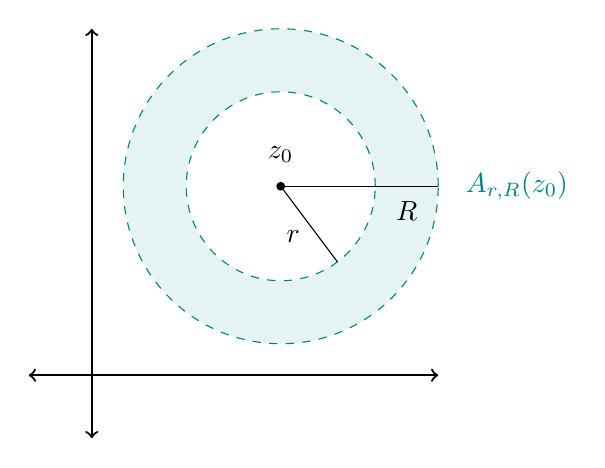
\begin{tikzpicture}[scale=0.8]
    \draw[<->,thick] (-1,0)--(5.5,0);
	\draw[<->,thick] (0,-1)--(0,5.5);
	\filldraw[teal,fill opacity=1/10,dashed](3,3) circle (2.5);
	\fill[white](3,3) circle (1.5);
    \draw[teal,dashed](3,3) circle (1.5);
    \draw[](3,3)--(5.5,3);
    \draw[](3,3)--(3.9,1.8);
    \fill (3,3) circle (2pt);
    \node[] at (3,3.5) {$z_0$};
    \node[] at (6.75,3) {\color{teal}$A_{r,R}(z_0)$};
    \node[] at (5,2.6) {$R$};
    \node[] at (3.2,2.2) {$r$};
  \end{tikzpicture}\]
\end{itemize}
\end{discussion}

%\vspace*{0.2in}

\subsection{Problems}
\vspace{0.1in}

\begin{problem}[]\label{prob 1.1a}
Consider the set of matrices
\[X \coloneqq \setp{\begin{pmatrix}x & -y\\ y & x \end{pmatrix}}{x,y \in \rr}.\]
One can check (and you should if you're unconvinced) straightforwardly that $X$ is closed under matrix addition and matrix multiplication; that is, if $A,B \in X$, then $A+B,\, AB \in X$.
\begin{itemize}[itemsep=1em]
\item[(a)] Let $\cc$ denote the set of complex numbers. Show that the map $\phi: X \to \cc$ defined by 
\[\phi:X \to \cc,\quad \begin{pmatrix}x & -y\\ y & x \end{pmatrix} \mapsto x + iy\]
is a bijection. 
\item[(b)] Let $I = \begin{pmatrix}1 & 0\\ 0 & 1\end{pmatrix}$ be the identity matrix. Consider $A,B \in X$, show that $\phi$ has the following properties.
\begin{itemize}[itemsep=1em]
\item[(i)] $\phi(A+B) = \phi(A)+\phi(B)$
\item[(ii)] $\phi(AB) = \phi(A)\phi(B)$
\item[(iii)] $\phi(I) = 1$
\end{itemize}
\item[(c)] Find a matrix $J$ satisfying $J^2 = -I$ and show that $\phi(J) = i$.
\end{itemize}
\vspace*{0.05in}
\begin{remark}
This indicates that one could very well define $\cc$ to be $X$. The algebraic operations on $\cc$ then seem less artificial, since product and sum of complex numbers correspond to the corresponding operations of matrices. Even taking the inverse and modulus is captured by $X$ as taking inverse and the determinant of matrices. The copy of $\rr$ corresponds to the set of diagonal matrices in $X$. One obtains $X$ by considering the linear operator of multiplying by $x + iy$ on the $\rr$-vector space $\cc$ with basis $1$ and $i$.
\end{remark}
\end{problem}

\vspace*{0.1in}

\begin{problem}\label{prob 1.1}
Using the definition of complex multiplication prove that
\[(a,0)\cdot (x,y) = (ax,ay).\]
That is, $a(x + iy) = ax + iay$.
\end{problem}

\vspace*{0.1in}

\begin{problem}\label{prob 1.2}
Consider complex numbers $z_1 = (x_1,y_1) = x_1(1,0) + y_1(0,1)$ and $z_2 = (x_2,y_2) = x_2(1,0) + y_2(0,1)$. Using the identity $(0,1)^2 = (-1,0)$. Prove that \[(x_1(1,0) + y_1(0,1))\cdot (x_2(1,0) + y_2(0,1)) = (x_1x_2 - y_1y_2, x_1y_2 + x_2y_1),\] where the former is computed distributively.
\end{problem}

\newpage
%\vspace*{0.1in}

\begin{problem}\label{prob 1.3}
Prove properties (1) - (7) and (9) listed in Proposition \ref{cafield}.
\end{problem}

\vspace*{0.1in}

\begin{problem}\label{prob 1.3a}
Prove that if $z_1z_2 = 0$, then $z_1 = 0$ or $z_2 = 0$.
\end{problem}

\vspace*{0.1in}

\begin{problem}\label{prob 1.4}
Show that
%\begin{multicols}{2}
\begin{itemize}
\item[(a)] $\Re iz = - \Im z$;
\item[(b)] $\Im iz = \Re z$
\end{itemize}
%\end{multicols}
\end{problem}

\vspace*{0.1in}

\begin{problem}\label{prob 1.5}\hfill
\begin{itemize}
\item[(a)] Verify that $z = 1 \pm i$ satisfies the equation \[z^2 - 2z + 2 = 0.\]
\item[(b)] Solve the equation \[z^2 + z + 1 = 0\] for $z = x + iy$ by solving a pair of simultaneous equations in $x$ and $y$.
\end{itemize}
\end{problem}

\vspace*{0.1in}

\begin{problem}\label{prob 1.5a}
Let $p(z) = az^2 + bz + c$ be a polynomial with complex coefficients ($a\neq 0$). 
\begin{itemize}
\item[(a)] By completing the square, show that the solution to $p(z) = 0$ is
\[z = \frac{-b \pm \Delta^{1/2}}{2a},\]
where $\Delta \coloneqq b^2 - 4ac$ is called the discriminant.\\[0.5em]
{\footnotesize Remark. There's a subtlety with taking roots that we will address later in class.}
\item[(b)] Consider the polynomial $p(z) = iz^2 -1$
\begin{itemize}
\item[(i)] Compute $\Delta$.
\item[(ii)] For the $\Delta$ obtained in (b), compute $\Delta^{1/2}$ by solving a pair of simultaneous equations in $x$ and $y$ obtained by considering the equation \[x^2 - y^2 + 2ixy = (x + iy)^2 = \Delta.\]
\item[(iii)] Finally, write down the roots of $p(z)$ in the form $u + iv$.
\end{itemize}
\end{itemize}
\end{problem}

\vspace*{0.1in}

\begin{problem}\label{prob 1.6}
Suppose $\cc$ had total ordering that extends the ordering on $\rr$, arrive at a contradiction by comparing $i$ and $0$.
\end{problem}

\vspace*{0.1in}

\begin{problem}\label{prob 1.7}
Locate the numbers $z_1 + z_2,\, z_1 - z_2$ and $z_1z_2$ in the complex plane when
\begin{multicols}{2}
\begin{itemize}
\item[(a)] $z_1 = 2i,\, z_2 = \dfrac{2}{3} - i$.
\item[(b)] $z_1 = (-3,1),\,z_2 = (1,4)$.
\item[(c)] $z_1 = (-\sqrt{3},1),\,z_2 = (\sqrt{3},0)$.
\item[(d)] $z_1 = x_1 + iy_1,\,z_2 = x_1 - iy_1$.
\end{itemize}
\end{multicols}
\end{problem}

\vspace*{0.1in}

\begin{problem}\label{prob 1.8}
Verify that $\sqrt{2}\abs{z} \geq \abs{\Re z} + \abs{\Im z}$.
\end{problem}

\vspace*{0.1in}

\begin{problem}\label{prob 1.9}
Let $z_0\neq z_1 \in \cc$ and let $\lambda >0$.
\begin{itemize}[itemsep=1em]
\item[(a)] Show that if $\lambda \neq 1$, then the set of points
\begin{equation*}\label{par}
\abs{z-z_0} = \lambda \abs{z-z_1}\tag{$\bigstar$}
\end{equation*}
is a circle of radius $R = \dfrac{\lambda}{\abs{1-\lambda^2}} \abs{z_0 - z_1}$ centered at $w = \dfrac{z_0 - \lambda^2 z_1}{1-\lambda^2}$.\\[0.5em]
\item[(b)] Show that every circle in the complex plane can be written in the form of (\ref{par}) for some $\lambda >0,\, \lambda \neq 1$ and $z_0 \neq z_1 \in \cc$. 
\item[(c)] If $\lambda = 1$, show that (\ref{par}) defines a line. In fact, argue that the resulting line is perpendicular to and bisects the line segment joining $z_0$ and $z_1$, by producing the equation of this line as a subset of $\rr^2$.
\item[(d)] Characterise points on the real (resp. imaginary) axis using (c). That is, find $z_0 \neq z_1 \in \cc$ such that the points on the real (resp. imaginary) axis satisfy (\ref{par}) for $\lambda = 1$.
\item[(e)] Consider the map \[M(z) = \dfrac{z-3}{1 - 2z}.\] For which values of $c \in \rr$ is the image of the circle $\abs{z - 1} = c$ under $M$ a line? What is the equation of the line when considered as a subset of the plane $\rr^2$?
\end{itemize}
\end{problem}